%----------------------------------------------------%
%              DISEÑO E IMPLEMENTACIÓN               %
%----------------------------------------------------%

\chapter{Diseño e Implementación}
\label{diseno-e-implementacion}

En este capítulo se comienza detallando la estructura de ficheros y carpetas del proyecto en el apartado \ref{diseno-e-implementacion:estructura}. Seguidamente tenemos dos apartados importantes: el \ref{diseno-e-implementacion:interfaces} en el que se muestran las interfaces y, en general, el lado cliente y el \ref{diseno-e-implementacion:logica-negocio} en el que se muestra la lógica de negocio.\\

\section{Estructura del proyecto}
\label{diseno-e-implementacion:estructura}

En este apartado se revisara la estructura del proyecto, es decir, los ficheros que componen el proyecto y su estructura de carpetas. En la figura ~\ref{fig:files-1} se muestra la raíz del proyecto:\\

\begin{figure}[h]
	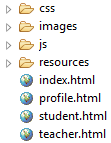
\includegraphics{files-1}
	\caption{Raíz del proyecto}
	\label{fig:files-1}
\end{figure}

El proyecto cuenta con 4 carpetas principales: css, js, images y resources. Además contiene 4 ficheros HTML:

\begin{itemize}
\item \textbf{index.html:} funciona como pantalla de identificación de usuario y permite redirigir a las vistas principales (teacher.html o student.html) dependiendo del rol del usuario identificado.
\item \textbf{student.html:} es la vista del alumno.
\item \textbf{teacher.html:} es la vista del profesor.
\item \textbf{profile.html:} pantalla de perfil del profesor, únicamente accesible desde teacher.html.
\end{itemize}

Estos ficheros muestran las interfaces principales de la aplicación. Dentro de las otras carpetas encontramos más ficheros.

\begin{figure}[h]
\begin{subfigure}[b]{0.5\textwidth}
	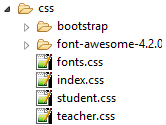
\includegraphics[width=0.6\linewidth]{files-css}
	\caption{Contenido de la carpeta css}
	\label{fig:files-css}
\end{subfigure}
%
\begin{subfigure}[b]{0.5\textwidth}
	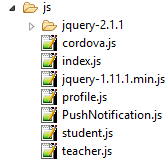
\includegraphics[width=0.6\linewidth]{files-js}
	\caption{Contenido de la carpeta js}
	\label{fig:files-js}
\end{subfigure}
%
\begin{subfigure}[b]{0.5\textwidth}
	
\includegraphics[width=0.6\linewidth]{files-images}
	\caption{Contenido de la carpeta images}
	\label{fig:files-images}
\end{subfigure}
%
\begin{subfigure}[b]{0.5\textwidth}
	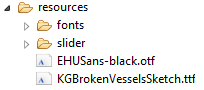
\includegraphics[width=0.6\linewidth]{files-resources}
	\caption{Contenido de la carpeta resources}
	\label{fig:files-resources}
\end{subfigure}

\caption{Contenido de la carpetas principales de la raíz del proyecto}
\label{fig:files-2}
\end{figure}

Los archivos de CSS sirve para darle estilo a las interfaces. Cada interfaz tiene un archivo .css asociado (excepto profile.html, que comparte teacher.css con teacher.html). Además, se añaden dos carpetas extra: la que necesitamos para Boostrap \hyperref[boostrap]{\cite{boostrap}} y para usar los iconos de Font Awesome \hyperref[fontawesome]{\cite{fontawesome}}.\\

Los ficheros Javascript de la carpeta JS le dan dinamicidad a la aplicación. Controlan los clicks, hacen aparecer las pestañas nuevas y cargan contenido dinámicamente mediante AJAX. Cada interfaz (fichero HTML) tiene asociado su propio fichero JS. Además se incluye el fichero cordova.js y los ficheros necesarios para utilizar JQuery.\\

La carpeta images contiene las imágenes utilizadas en el proyecto y la carpeta resources contiene otros elementos utilizados en el proyecto (en este caso fuentes utilizadas).\\

\section{Interfaces o lado del cliente}
\label{diseno-e-implementacion:interfaces}

En este apartado se mostrarán las interfaces desarrolladas partiendo de los modelos de requisitos (M-1) de cada objetivo y algunos elementos comunes de todos los objetivos.

\subsection{Interfaz de autenticación de usuario}
\label{diseno-e-implementacion:interfaces:autenticacion}

\begin{figure}[H]
	\centering
	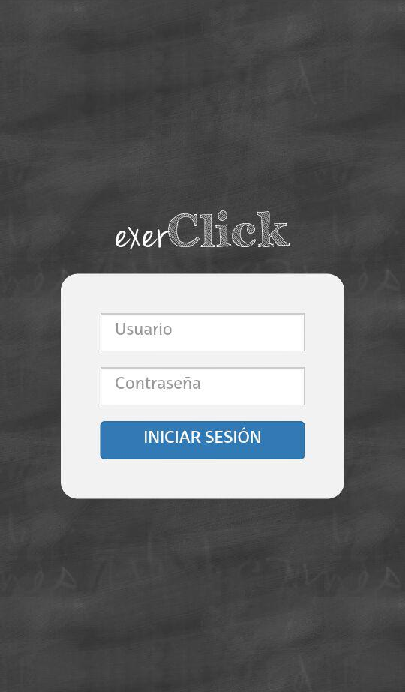
\includegraphics[height=7cm, frame]{autenticacion}
	\caption{Pantalla de autenticación de usuario}
	\label{fig:autenticacion}
\end{figure}

La pantalla de autenticación de usuario (index.html) de la figura ~\ref{fig:autenticacion} es la primera que se muestra al iniciar la aplicación. Esta pantalla nos redirige a teacher.html o student.html (vista del profesor y del alumno, respectivamente) dependiendo del rol del usuario con el que nos identifiquemos (el rol está definido en la base de datos).\\

\subsection{Interfaz del profesor}
\label{diseno-e-implementacion:interfaces:profesor}

\begin{figure}[H]
	\centering
	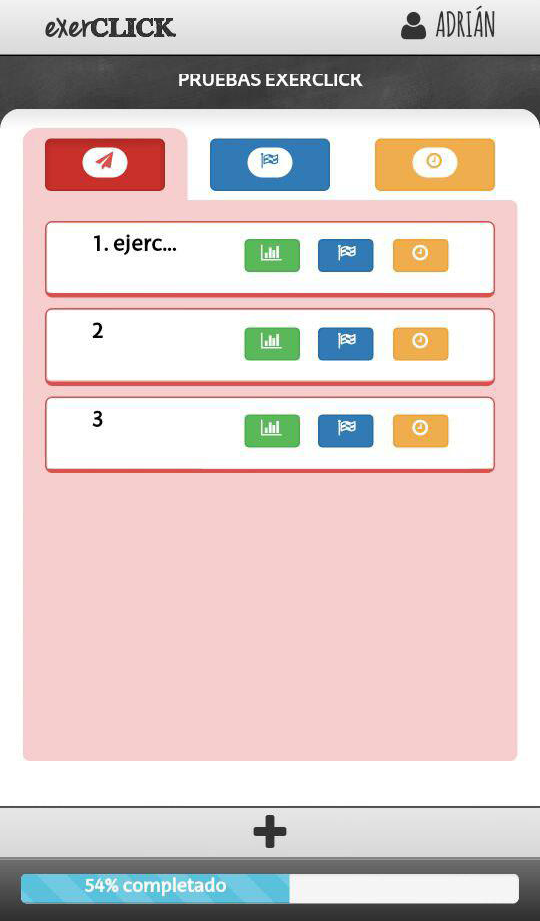
\includegraphics[height=7cm, frame]{activos}
	\caption{Pantalla en la que se muestran los ejercicios activos en clase}
	\label{fig:activos}
\end{figure}

La pantalla del profesor nos muestra el entorno de opciones del que dispone el docente.\\

\subsection{Interfaz del perfil del profesor}
\label{diseno-e-implementacion:interfaces:perfil}

\begin{figure}[H]
	\centering
	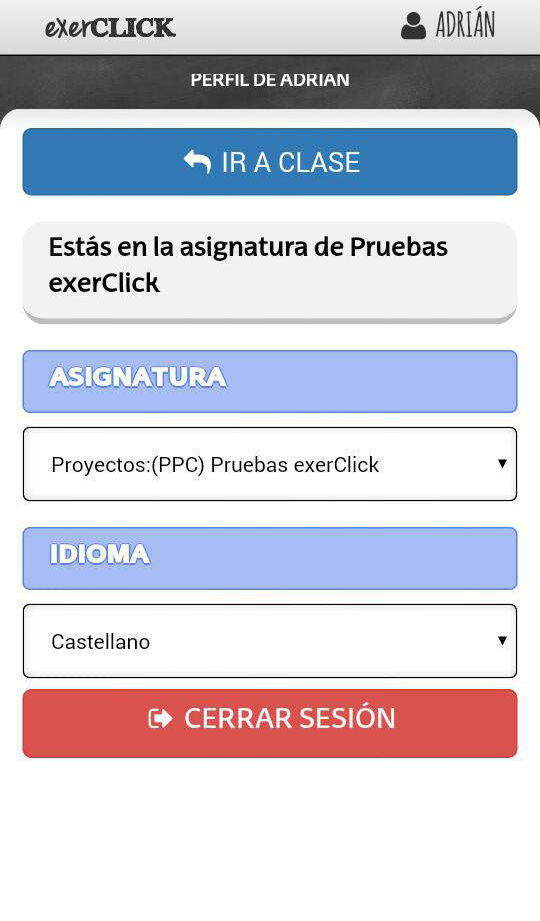
\includegraphics[height=7cm, frame]{perfil}
	\caption{Perfil del profesor}
	\label{fig:perfil}
\end{figure}

Es la interfaz de teacher.html, y la vista de profesor de inicio después de autenticarse. Esta pantalla sirve como base de cualquier UO del profesor, ya que hay que pasar obligatoriamente por ella.

\subsubsection{UO1-T: Crear-Lanzar un ejercicio simple}
\label{diseno-e-implementacion:interfaces:profesor:uo1-t}

\begin{figure}[H]
	\centering
	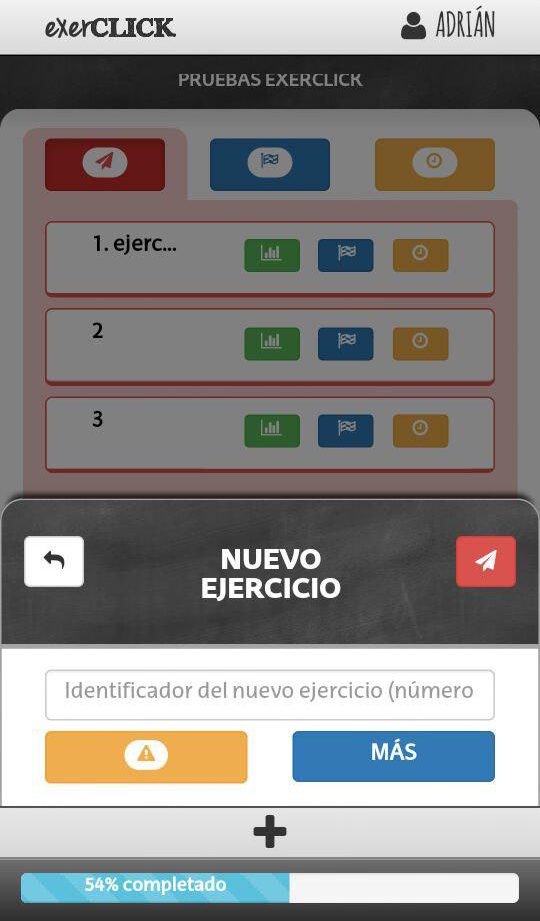
\includegraphics[height=7cm, frame]{ejercicio-simple}
	\caption{Interfaz del UO1-T: Crear-Lanzar un ejercicio simple}
	\label{fig:crear-lanzar-ejercicio-simple}
\end{figure}

Al pulsar el botón con símbolo de '+' (\textit{plus}/más) de la parte inferior de la interfaz del profesor se desplegará la pestaña que aparece en la figura ~\ref{fig:crear-lanzar-ejercicio-simple}.

\subsubsection{UO2-T: Crear-Lanzar un ejercicio detallado}
\label{diseno-e-implementacion:interfaces:profesor:uo2-t}

\begin{figure}[H]
	\centering
	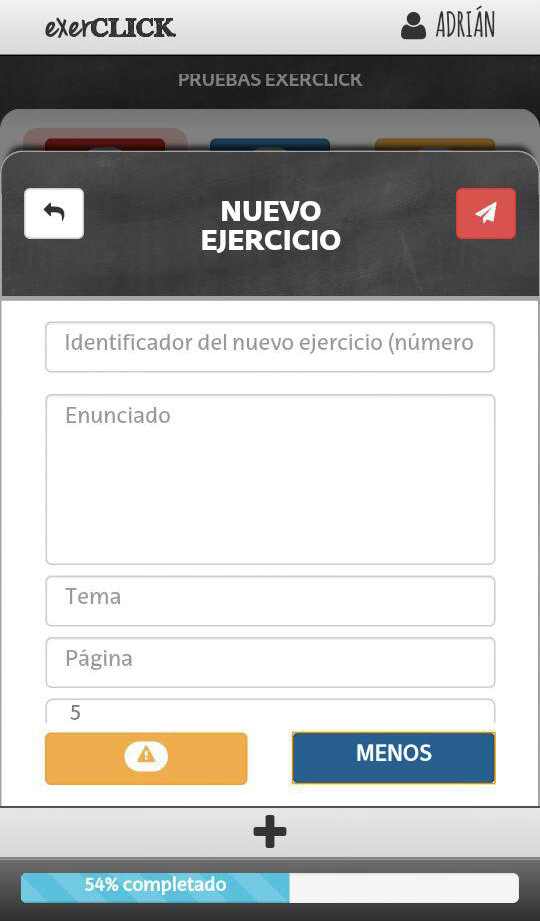
\includegraphics[height=7cm, frame]{ejercicio-avanzado}
	\caption{Interfaz del UO1-T: Crear-Lanzar un ejercicio detallado}
	\label{fig:crear-lanzar-ejercicio-avanzados}
\end{figure}

\subsubsection{UO4-T: Ver estadísticas de un ejercicio}
\label{diseno-e-implementacion:interfaces:profesor:uo4-t}

\begin{figure}[H]
\begin{subfigure}[b]{0.3\textwidth}
	\centering
	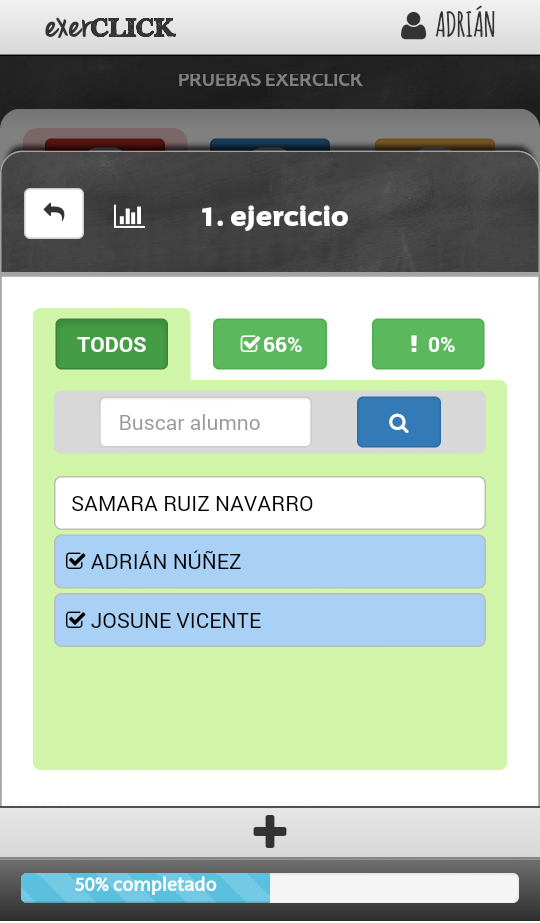
\includegraphics[height=7cm, frame]{P5T}
	\caption{P5T}
	\label{fig:req-autenticacion:p0}
\end{subfigure}
%
\begin{subfigure}[b]{0.3\textwidth}
	\centering
	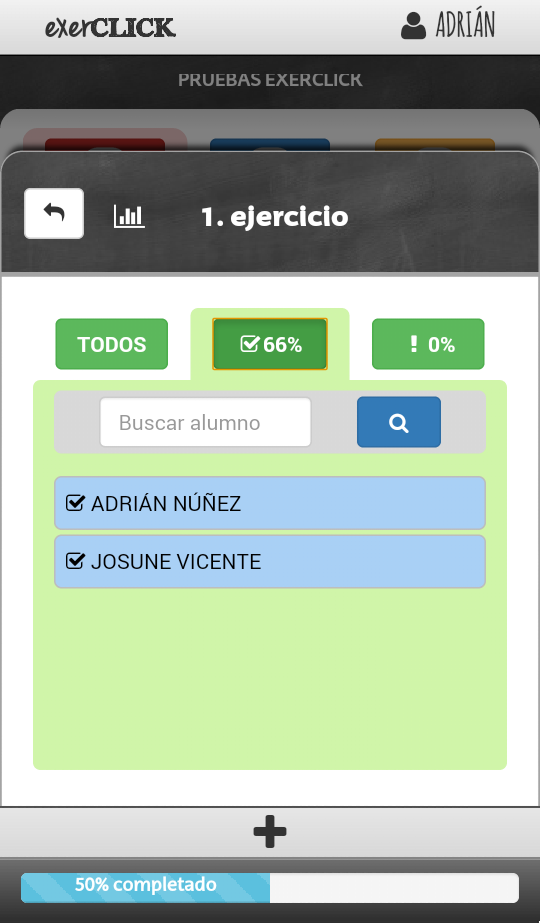
\includegraphics[height=7cm, frame]{P5A}
	\caption{P5A}
	\label{fig:req-autenticacion:p0'}
\end{subfigure}
%
\begin{subfigure}[b]{0.3\textwidth}
	\centering
	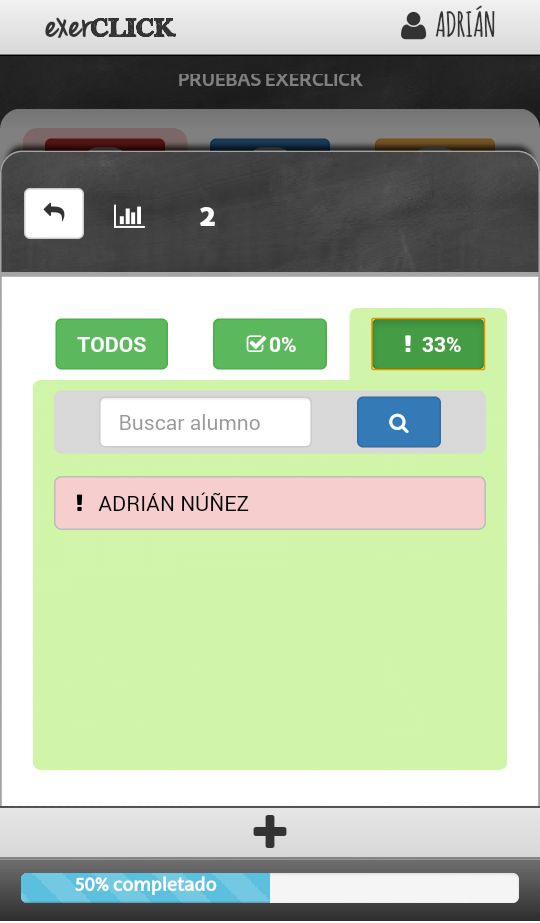
\includegraphics[height=7cm, frame]{P5D}
	\caption{P5D}
	\label{fig:fsm-autenticacion}
\end{subfigure}

\label{fig:autenticacion}
\end{figure}

\subsubsection{UO5-T: Ver la descripción completa de un ejercicio}
\label{diseno-e-implementacion:interfaces:profesor:uo5-t}

\begin{figure}[H]
	\centering
	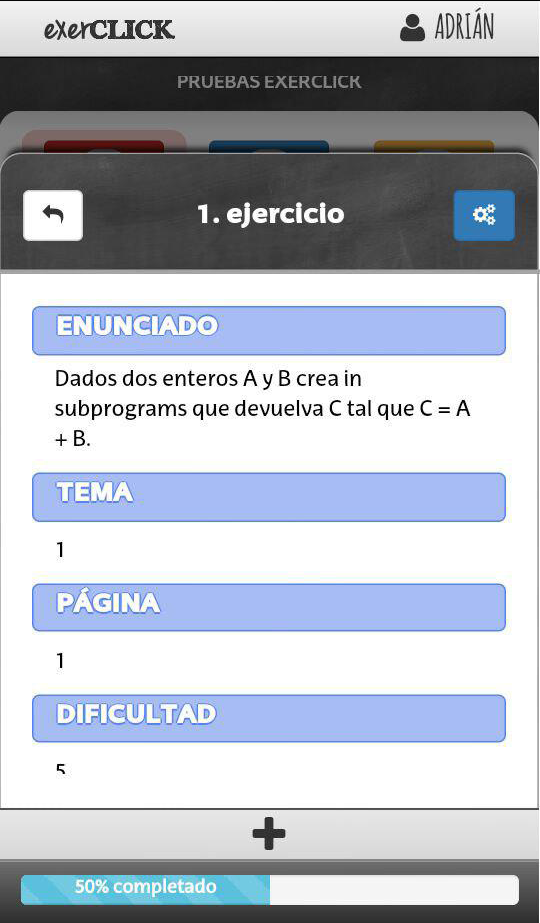
\includegraphics[height=7cm, frame]{P3}
	\caption{P3}
	\label{diseno-e-implementacion:interfaces:profesor:uo5-t:p3}
\end{figure}

\subsubsection{UO6-T: Editar un ejercicio}
\label{diseno-e-implementacion:interfaces:profesor:uo6-t}

\begin{figure}[H]
\begin{subfigure}[b]{0.3\textwidth}
	\centering
	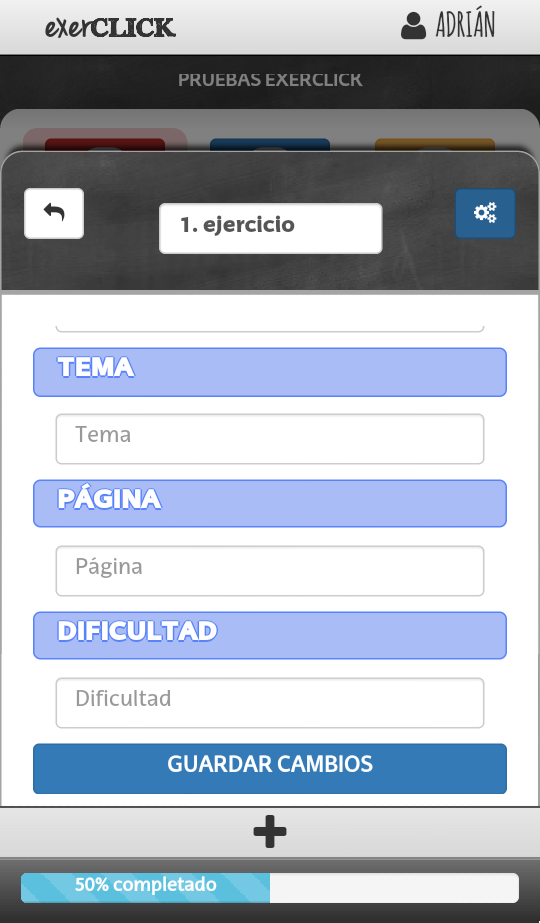
\includegraphics[height=7cm, frame]{P4}
	\caption{P5T}
	\label{fig:req-autenticacion:p0}
\end{subfigure}
%
\begin{subfigure}[b]{0.3\textwidth}
	\centering
	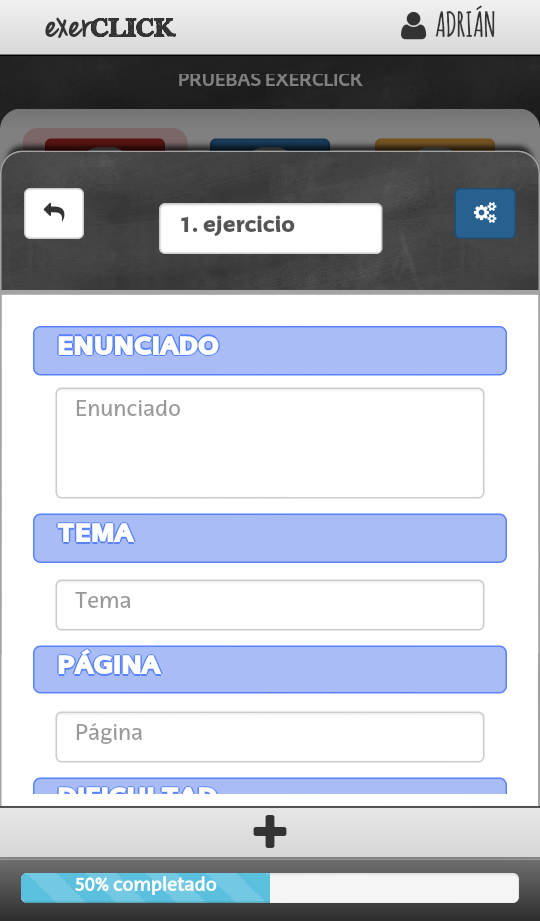
\includegraphics[height=7cm, frame]{P4-2}
	\caption{P5A}
	\label{fig:req-autenticacion:p0'}
\end{subfigure}
%
\begin{subfigure}[b]{0.3\textwidth}
	\centering
	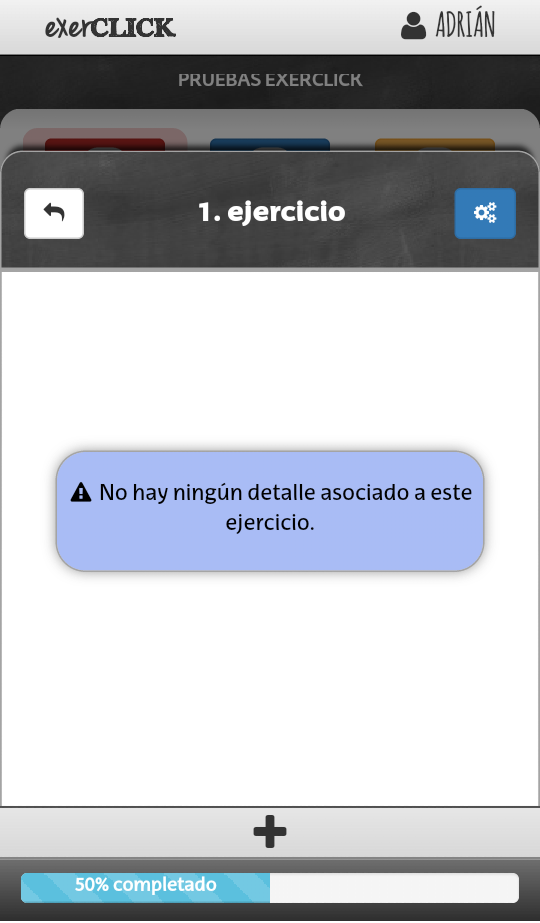
\includegraphics[height=7cm, frame]{P4'}
	\caption{P5D}
	\label{fig:fsm-autenticacion}
\end{subfigure}

\label{fig:autenticacion}
\end{figure}

\subsection{Interfaz del alumno}
\label{diseno-e-implementacion:interfaces:alumno}

\begin{figure}[H]
	\centering
	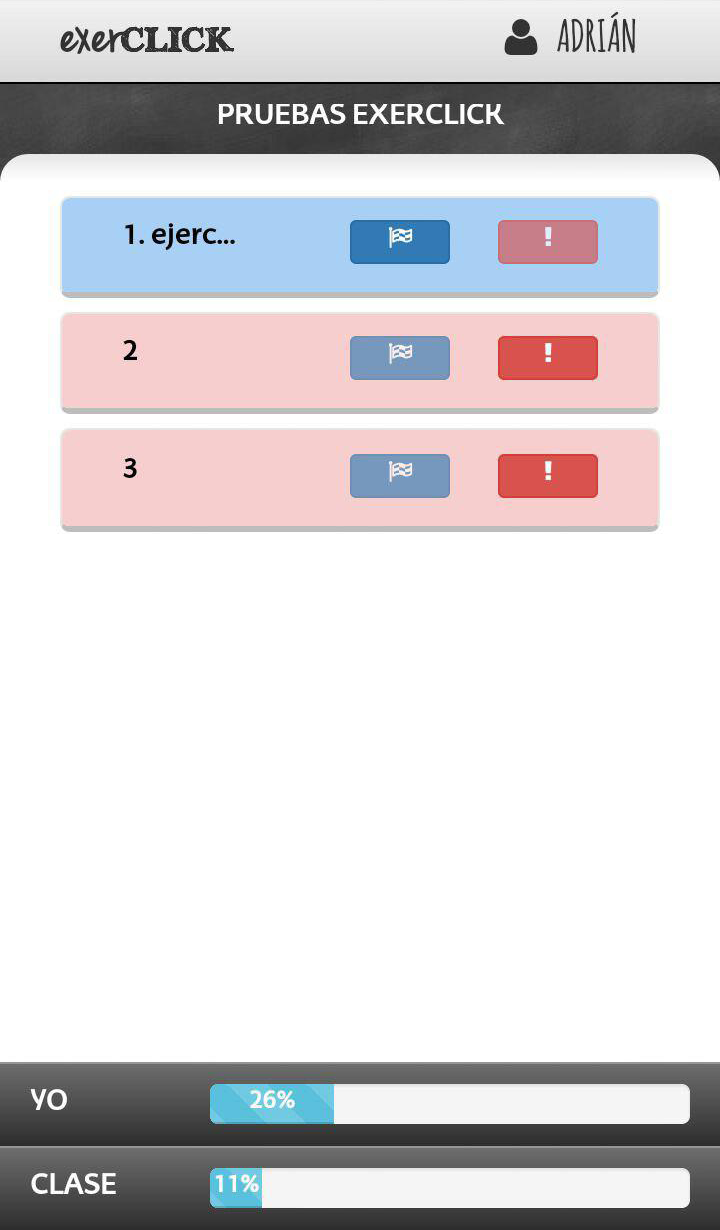
\includegraphics[height=7cm, frame]{P1-S}
	\caption{P1}
	\label{diseno-e-implementacion:interfaces:alumno:p1}
\end{figure}

La pantalla del alumno le muestra a este el estado actual de la clase: los ejercicios activos, su progreso en esta sesión y la media de progreso de la clase.

\subsubsection{UO1-S: Responder a un ejercicio}
\label{diseno-e-implementacion:interfaces:alumno:uo1-s}

\begin{figure}[H]
\begin{subfigure}[b]{0.3\textwidth}
	\centering
	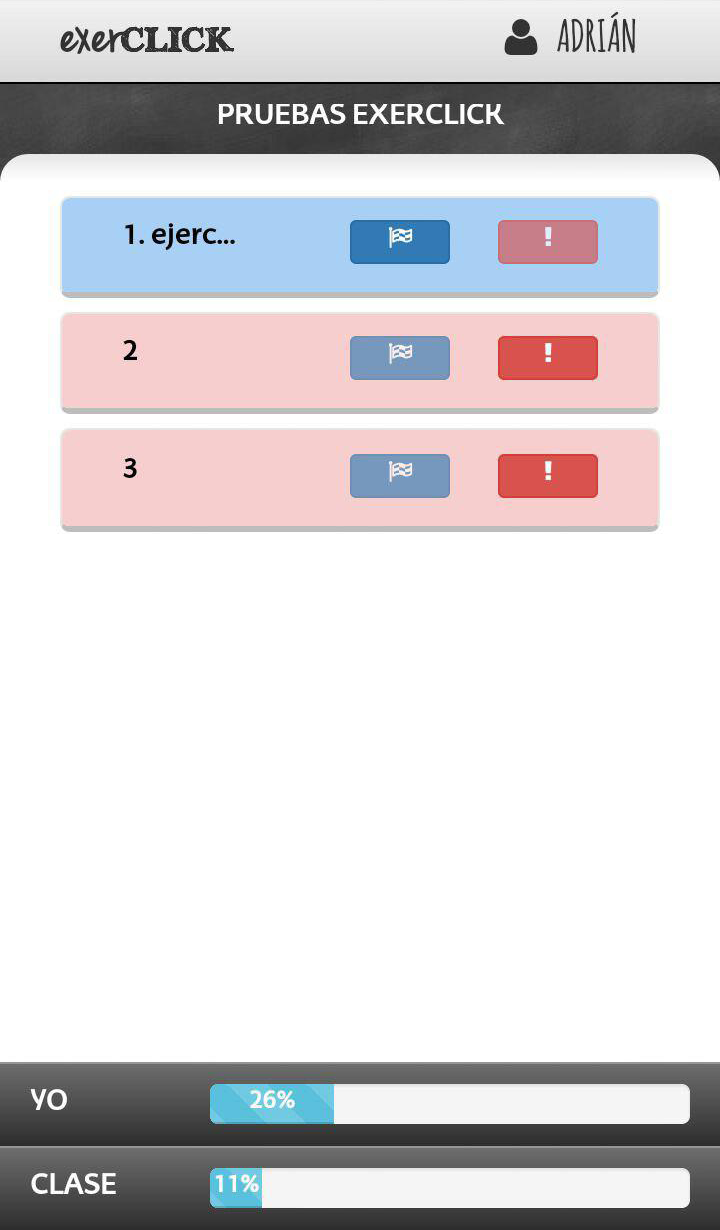
\includegraphics[height=7cm, frame]{P1-S}
	\caption{P1}
	\label{diseno-e-implementacion:interfaces:alumno:p1}
\end{subfigure}
%
\begin{subfigure}[b]{0.3\textwidth}
	\centering
	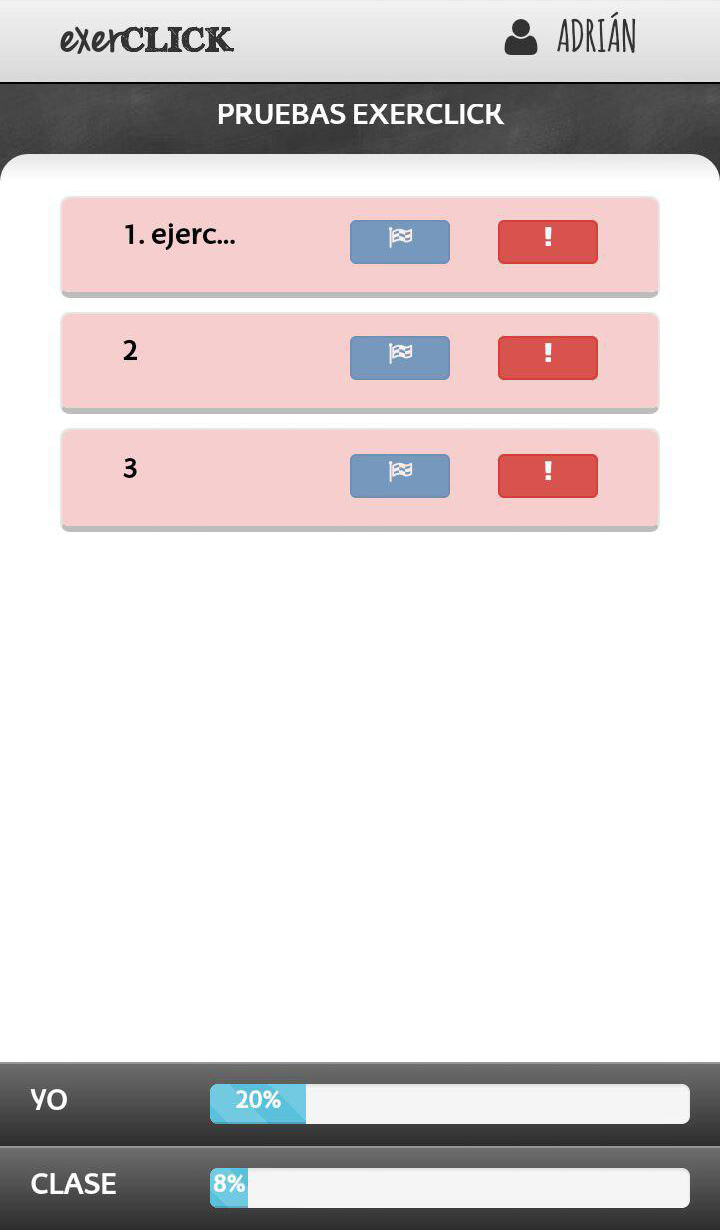
\includegraphics[height=7cm, frame]{P1-S'}
	\caption{P1'}
	\label{diseno-e-implementacion:interfaces:alumno:p1'}
\end{subfigure}

\label{fig:p1-student}
\end{figure}

\subsubsection{UO2-S: Ver detalles de un ejercicio}
\label{diseno-e-implementacion:interfaces:alumno:uo2-s}

\begin{figure}[H]
	\centering
	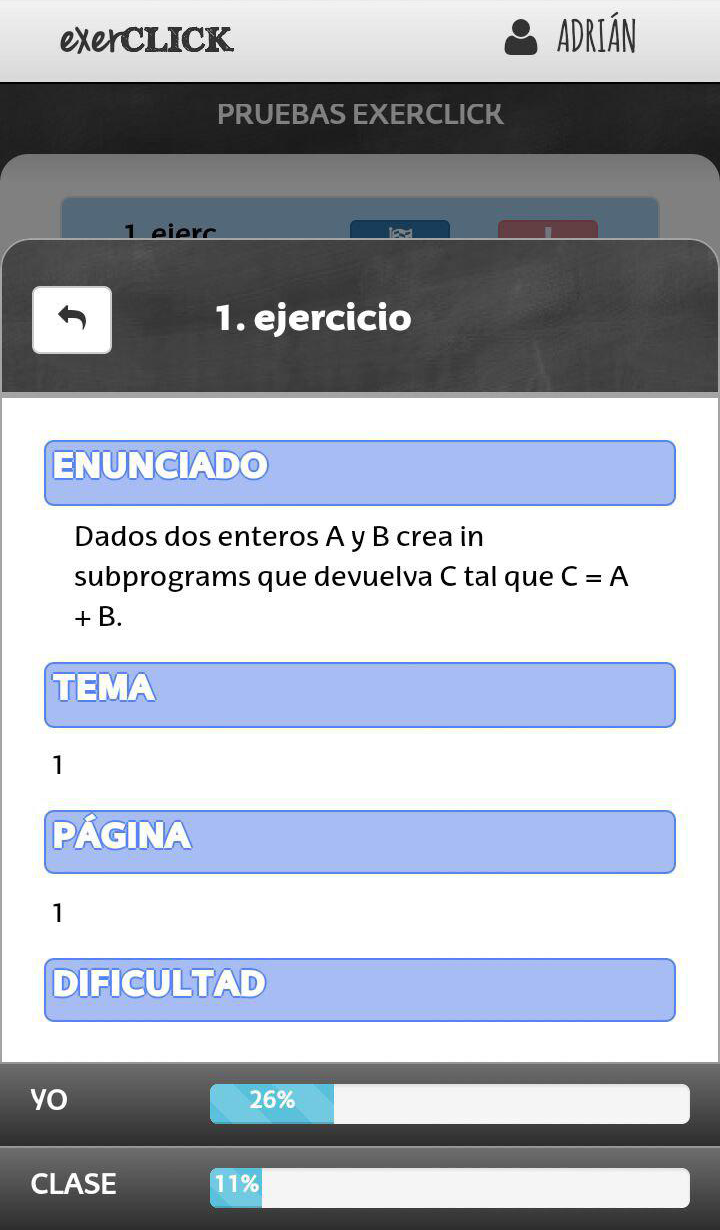
\includegraphics[height=7cm, frame]{P2-S}
	\caption{P2}
	\label{diseno-e-implementacion:interfaces:alumno:p1}
\end{figure}

\subsection{Uso de iconos mediante Font Awesome}
\label{diseno-e-implementacion:interfaces:font-awesome}

Font Awesome \hyperref[fontawesome]{\cite{fontawesome}} es un sitio web generado mediante un repositorio de Github. De este sitio se han obtenido todos los iconos de la aplicación: desde los iconos de los botones hasta el icono de usuario que aparece junto al nombre de usuario.\\

Su uso es sencillo, para añadir cualquier icono basta con añadir código como el de este ejemplo (para añadir el icono del avión de papel de los ejercicios activos):\\

\begin{lstlisting}[frame=single]
<i class="fa fa-paper-plane"></i>
\end{lstlisting}

Además podemos aumentar el tamaño del icono añadiendo clases del tipo fa-2x, fa-3x, etc. (aumentan por 2 y por 3 el tamaño del icono, respectivamente). También existe la opción de adaptarlo al texto que tiene cerca con fa-fw y otras tantas opciones que no se han llegado a utilizar en el proyecto (rotaciones, añadir un marco de prohibido encima, etc.). Se pueden encontrar ejemplos en la propia página.\\

\section{Lógica de negocio o lado del servidor}
\label{diseno-e-implementacion:logica-negocio}

Hablar sobre la parte de servidor y la base de datos.\\

\subsection{Base de datos}
\label{diseno-e-implementacion:logica-negocio:bd}

El diseño de la base de datos se ha realizado considerando desarrollos anteriores del grupo GaLan.
Por ello muchos de los elementos son comunes con una de sus herramientas genérica de creación
de sistemas docente, MAGADI, que ha sido proporcionada para este proyecto.\\

Se han incorporado unas tablas nuevas a la base de datos ya existente para la gestión de ejercicios tal y como se muestra en la figura ~\ref{fig:base-de-datos} del apéndice C.\\


\subsection{Configuración}
\label{diseno-e-implementacion:configuracion}

\noindent
\begin{lstlisting}[caption=Autenticación del usuario.,label={lst:autenticacion}]
<?php
	define('HOST', 'xxxx');
	// Database username
	define('USER', 'xxxx');
	// Database password
	define('PASSWORD', 'xxxx');
	// Database name
	define('DATABASE', 'xxxx'); 
	 
	define("CAN_REGISTER", "any");
	define("DEFAULT_ROLE", "member");
?>
\end{lstlisting}

Este archivo de configuración define datos de autenticación en la base de datos. Se añade y utiliza en cada fichero mediante el siguiente código:

\noindent
\begin{lstlisting}[caption=Autenticación del usuario.,label={lst:autenticacion}]
include 'mysqli-config.php';
$mysqli = new mysqli(HOST, USER, PASSWORD, DATABASE);

if (mysqli_connect_errno()) {
     echo "Failed to connect to MySQL: " . mysqli_connect_error();
}
\end{lstlisting}

Este trozo de código se añade siempre al inicio de cada código PHP en el servidor. Al final se cierra la base de datos.\\

\subsection{Identificación de usuario}
\label{diseno-e-implementacion:logica-negocio:identificacion}

\noindent
\begin{lstlisting}[caption=Autenticación del usuario.,label={lst:autenticacion}]
$name = test_input($_GET['Username']);
$pass = test_input($_GET['Password']);
   
// Check if username exists
$statement = 'SELECT * FROM fos_user WHERE username="' . $name . '"'; 
$result = $mysqli->query($statement);

// Only 1 result, otherwise error
$num = mysqli_num_rows($result);
if($num != 1){
     die();
}

$row = mysqli_fetch_assoc($result);
if(!isPasswordValid($row['password'], $pass, $row['salt'])) {
     die();
}
// Mandatory call for using $_SESSION array
session_start();
$_SESSION['name'] = $row['username'];

// Check for the role of the user
if (strpos($row['roles'], 'ROLE_STUDENT') !== false) {
     $_SESSION['role'] = "ROLE_STUDENT";
}
if (strpos($row['roles'], 'ROLE_TEACHER') !== false) {
     $_SESSION['role'] = "ROLE_TEACHER";
}

// Save the user id
$_SESSION['general_id'] = $row['id'];
  
// Find id based in role
switch($_SESSION['role']) {
case 'ROLE_STUDENT':
     $statement = 'SELECT id, name, surname1, surname2 FROM student WHERE fosUser="' . $row['id'] . '"';
     $next_location = 'student.html';
     break;	
case 'ROLE_TEACHER':
     $statement = 'SELECT id, name, surname1, surname2 FROM teacher WHERE fosUser="' . $row['id'] . '"';
     $next_location = 'teacher.html';
     break;
}    

$result = $mysqli->query($statement);
if(!$result) {
     die('The query has encounter a problem: ' . mysqli_error($mysqli));
}
  
// Only 1 result, otherwise error
$num = mysqli_num_rows($result);
if($num != 1){
     session_destroy();
     die('No role asigned.');
}
\end{lstlisting}

El código \ref{lst:autenticacion} se ejecuta en la interfaz P0 al intentar autenticarse. No se puede tener más de una sesión abierta en diferentes dispositivos, sólo la última sesión es la que se puede utilizar. En la base de datos proporcionada teníamos la tabla \textit{usersession} para almacenar las sesiones y mantener ese control. En esta tabla guardamos el ID de usuario global (almacenado en la tabla \textit{fosUser}) y el identificador de sesión generado por PHP. Además, dependiendo del rol del usuario se le llevará a la interfaz teacher.html o student.html.\\


\subsection{Cargar la interfaz principal (P1 del profesor y P1 del alumno)}
\label{diseno-e-implementacion:logica-negocio:carga}

\noindent
\begin{lstlisting}[caption=Obtener información inicial para la carga de la interfaz.,label={lst:get-data}]
if(!isset($_SESSION['class'])) {
     $now = date('H:i');
     $day = date('Y-m-d');
     // Find all classes previous to the actual time
     $statement = 'SELECT * FROM attendanceclass WHERE day <= "' . $day . '" OR (day = "' . $day . '" AND endHour < "' . $now . '") ORDER BY day DESC, startHour DESC';
		
     if(!($result = $mysqli->query($statement))) {
         die('The query has encounter a problem: ' . mysqli_error($mysqli));
     }
		
     $class = -1;
     while($row =  mysqli_fetch_array($result)) {
         // For the next class previous to the actual time find a session given by the logged teacher
         $statement = 'SELECT session.* FROM session INNER JOIN groupteacher ON session.ctGroup = groupteacher.ctGroup WHERE session.id = "' . $row['session'] . '" AND groupteacher.teacher= "' . $_SESSION['id'] . '"';
         if(!($session = $mysqli->query($statement))){
		      die('The query has encounter a problem: ' . mysqli_error($mysqli));
         }
         $group = mysqli_fetch_array($session);
         if(mysqli_num_rows($session) != 0){
              break;
         }
     }
     // Id of the session (next class)
     $class = $row['id'];
} else {
     $class = $_SESSION['class'];
     $statement = 'SELECT * FROM attendanceclass WHERE id= "' . $_SESSION['class'] . '"';
	  
     if(!($result = $mysqli->query($statement))){
          die('The query has encounter a problem: ' . mysqli_error($mysqli));
     }

     $row =  mysqli_fetch_array($result);
     $start = date('H:i', strtotime($row['startHour']));
     $end = date('H:i', strtotime($row['endHour']));
     $day = $row['day'];
}

if($_SESSION['role'] == 'ROLE_TEACHER') {
     $statement = 'SELECT subject.id, subject.name AS subject, subject.acronym, ctgroup.name, ctgroup.id AS group_id FROM subject INNER JOIN ctgroup ON ctgroup.subject = subject.id INNER JOIN groupteacher ON groupteacher.ctgroup = ctgroup.id WHERE groupteacher.teacher= "' . $_SESSION['id'] . '" ORDER BY subject.name ASC';
     if(!($subjects = $mysqli->query($statement))) {
	      die('The query has encounter a problem: ' . mysqli_error($mysqli));
     }
     $subj = array();
     while($row = mysqli_fetch_array($subjects)) {
          $subj[] = array('name' => $row['subject'], 'acronym' => $row['acronym'], 'group' => $row['name'], 'group_id' => $row['group_id'], 'id' => $row['id']);
     }
}
\end{lstlisting}

Es importante al cargar la interfaz saber si tenemos clase o no. Se utiliza principalmente el código \ref{lst:get-data} para ello. Si no hay ninguna guardada en la sesión abierta buscamos si en el día y hora en la que nos encontramos hay alguna clase. Si la hay guardamos el identificador de su \textit{attendanceclass}. En caso de que haya una clase activa simplemente obtendremos datos de ella (hora de inicio, de final y día).\\

Si nos hemos autenticado con el rol de profesor también obtendremos todas sus asignaturas, de modo que podamos cargarlas en el perfil del profesor más adelante.\\

\noindent
\begin{lstlisting}[caption=Cargar los ejercicios del tipo pasado por parámetro.,label={lst:carga-ejercicios}]
if($_SESSION['role'] == 'ROLE_TEACHER') {
     $statement = 'SELECT exercise.id, description FROM exercise LEFT JOIN ctgroup ON exercise.ctGroup = ctgroup.id INNER JOIN groupteacher ON groupteacher.ctgroup = ctgroup.id ' .
                           'WHERE type = "' . $_GET['Type'] . '" AND ctgroup.id = "' . $_SESSION['group_id'] . '" AND ctgroup.subject = "' . $_SESSION['subject_id'] . '" AND groupteacher.teacher = "' . $_SESSION['id'] . '"';
} else if($_SESSION['role'] == 'ROLE_STUDENT') {
     $statement  = 'SELECT exercise.id, description, state FROM exercise INNER JOIN ctgroup ON ctgroup.id = exercise.ctGroup INNER JOIN groupstudent ON groupstudent.ctgroup = exercise.ctgroup ' .
                           'INNER JOIN exercisestate ON exercise.id = exercisestate.idexercise WHERE type = "Active" AND exercisestate.idstudent = "' . $_SESSION['id'] . '" AND ctgroup.subject = "' . $_SESSION['subject_id'] . '" AND exercise.ctGroup = "' . $_SESSION['group_id'] . '" AND groupstudent.student = "' . $_SESSION['id'] . '"';
}

$result = $mysqli->query($statement);

$exercises = array();
while ($row = $result->fetch_assoc()) {
     $statement = 'SELECT * FROM exercise INNER JOIN exercisestate ON exercise.id = exercisestate.idexercise INNER JOIN ctgroup ON ctgroup.id = exercise.ctGroup ' .
                           'WHERE exercise.id = "' . $row['id'] . '" AND state = "Finished" AND ctgroup.id = "' . $_SESSION['group_id'] . '" AND ctgroup.subject = "' . $_SESSION['subject_id'] . '"';
     $result2 = $mysqli->query($statement);

     $statement = 'SELECT * FROM exercise INNER JOIN exercisestate ON exercise.id = exercisestate.idexercise INNER JOIN ctgroup ON ctgroup.id = exercise.ctGroup ' .
                           'WHERE exercise.id = "' . $row['id'] . '" AND state = "Question" AND ctgroup.id = "' . $_SESSION['group_id'] . '" AND ctgroup.subject = "' . $_SESSION['subject_id'] . '"';
     $result3 = $mysqli->query($statement);

     $statement = 'SELECT * FROM exercise INNER JOIN attendanceclass ON exercise.launched = attendanceclass.id INNER JOIN attendanceclassstudent ON attendanceclassstudent.attendanceclass = attendanceclass.id WHERE exercise.id = "' . $row['id'] . '"';
     $result4 = $mysqli->query($statement);
               
     $row['nofinished'] = mysqli_num_rows($result2);
     $row['noquestions'] = mysqli_num_rows($result3);
     $row['num'] = mysqli_num_rows($result4);
                
     $exercises[] = array('exercise' => $row);
}
\end{lstlisting}

El segundo elemento principal al cargar las interfaces es la carga de los ejercicios (como se puede ver en el código \ref{lst:carga-ejercicios}. Se obtienen los ejercicios en los que estamos involucrados (porque estamos matriculados en esa asignatura como alumno o porque la impartimos como profesor). Después, independientemente del rol del usuario autenticado, obtenemos para cada ejercicio que hemos obtenido de la base de datos: el número de alumnos que lo han marcado como acabado, el número de ellos que han marcado una duda y el número de alumnos total involucrados en el ejercicio.\\

\noindent
\begin{lstlisting}[caption=Obtener información para la carga de la barra de progreso del profesor.,label={lst:progress-bar-info-teacher}]
$statement = 'SELECT * FROM exercise INNER JOIN ctgroup ON ctgroup.id = exercise.ctGroup ' .
                           'WHERE ctgroup.id = "' . $_SESSION['group_id'] . '" AND ctgroup.subject = "' . $_SESSION['subject_id'] . '" AND exercise.type != "Ready"';
$result = $mysqli->query($statement);
$total = mysqli_num_rows($result);

$statement = 'SELECT * FROM exercise INNER JOIN ctgroup ON ctgroup.id = exercise.ctGroup ' .
                           'WHERE ctgroup.id = "' . $_SESSION['group_id'] . '" AND ctgroup.subject = "' . $_SESSION['subject_id'] . '" AND exercise.type = "Finished"';
$result = $mysqli->query($statement);
$finished = mysqli_num_rows($result);
\end{lstlisting}

\noindent
\begin{lstlisting}[caption=Obtener información para la carga de la barra de progreso del estudiante.,label={lst:progress-bar-info-student}]
$statement  = 'SELECT * FROM exercise INNER JOIN ctgroup ON ctgroup.id = exercise.ctGroup INNER JOIN exercisestate ON exercisestate.idexercise = exercise.id ' .
                           'WHERE ctgroup.id = "' . $_SESSION['group_id'] . '" AND ctgroup.subject = "' . $_SESSION['subject_id'] . '" AND exercisestate.idstudent = "' . $_SESSION['id'] . '"';	
$result = $mysqli->query($statement);
$total = mysqli_num_rows($result);

$statement       = 'SELECT * FROM exercise INNER JOIN ctgroup ON ctgroup.id = exercise.ctGroup INNER JOIN exercisestate ON exercisestate.idexercise = exercise.id ' .
                           'WHERE ctgroup.id = "' . $_SESSION['group_id'] . '" AND ctgroup.subject = "' . $_SESSION['subject_id'] . '" AND exercisestate.idstudent = "' . $_SESSION['id'] . '" AND exercisestate.state = "Finished"';
$result = $mysqli->query($statement);
$finished = mysqli_num_rows($result);

$studentprogress = ($total == 0) ? 0 : intval($finished * 100 / $total);

$statement = 'SELECT * FROM attendanceclassstudent INNER JOIN attendanceclass ON attendanceclass.id = attendanceclassstudent.attendanceclass INNER JOIN session ON attendanceclass.session = session.id INNER JOIN ctgroup ON ctgroup.id = session.ctGroup INNER JOIN exercise ON exercise.ctGroup = ctgroup.id INNER JOIN exercisestate ON exercisestate.idexercise = exercise.id ' .
                     'WHERE ctgroup.id = "' . $_SESSION['group_id'] . '" AND ctgroup.subject = "' . $_SESSION['subject_id'] . '"';
$result = $mysqli->query($statement);
$total = mysqli_num_rows($result);

$statement = 'SELECT * FROM attendanceclassstudent INNER JOIN attendanceclass ON attendanceclass.id = attendanceclassstudent.attendanceclass INNER JOIN session ON attendanceclass.session = session.id INNER JOIN ctgroup ON ctgroup.id = session.ctGroup INNER JOIN exercise ON exercise.ctGroup = ctgroup.id INNER JOIN exercisestate ON exercisestate.idexercise = exercise.id ' .
                      'WHERE ctgroup.id = "' . $_SESSION['group_id'] . '" AND ctgroup.subject = "' . $_SESSION['subject_id'] . '" AND exercisestate.state = "Finished"';
$result = $mysqli->query($statement);
$finished = mysqli_num_rows($result);
\end{lstlisting}

Ambas interfaces principales también comparten las barras de progreso de la clase. Para obtener la información para cargarlas se ejecuta el código \ref{lst:progress-bar-info-teacher} en el caso del profesor y el \ref{lst:progress-bar-info-student} en el caso del alumno. Nos devuelven el porcentaje de carga para cada barra mediante simples divisiones.\\

\subsection{Responder a un ejercicio (UO1-S)}
\label{diseno-e-implementacion:logica-negocio:responder-ejercicio}

\noindent
\begin{lstlisting}[caption=Responder a un ejercicio.,label={lst:responder-ejercicio}]
$idexercise = $_GET['Idexercise'];
$idstudent = $_SESSION['id'];
$state = $_GET['State'];

$statement = 'SELECT state FROM exercisestate WHERE idexercise = "' . $idexercise . '" AND idstudent = "' . $idstudent . '"';
$result = $mysqli->query($statement);
$row = $result->fetch_assoc();
if($row['state'] == 'Question' && ($state == 'Nothing' || $state == 'Finished')) {
     $statement = 'SELECT * FROM exercise_solved_questions WHERE idexercise = "' . $idexercise . '" AND idstudent = "' . $idstudent . '"';
     $result = $mysqli->query($statement);
	
     $day = date('Y-m-d');
     $time = date('H:i:s');
     if(mysqli_num_rows($result) == 1) {
          $statement = 'UPDATE exercise_solved_questions SET day = "' . $day . '" AND time = "' . $time . '" WHERE idexercise = "' . $idexercise . '" AND idstudent = "' . $idstudent . '"';
          $mysqli->query($statement);
     } else {
          $statement = 'INSERT INTO exercise_solved_questions (idexercise, idstudent, day, time) VALUES ("' . $idexercise . '", "' . $idstudent . '", "' . $day . '", "' . $time . '")';
          $mysqli->query($statement);
     }
}
$statement = 'UPDATE exercisestate SET state = "' . $state . '" WHERE idexercise = "' . $idexercise . '" AND idstudent = "' . $idstudent . '"';
$result = $mysqli->query($statement);
\end{lstlisting}

Un alumno puede marcar un ejercicio como acabado o con una duda. Este nuevo estado s pasa por parámetro y se procesa con el código \ref{lst:responder-ejercicio}.\\

Si el ejercicio estaba con una duda marcada y la quitamos inmediatamente debemos guardarlo en la base de datos como una duda resuelta (estas dudas resueltas se muestran en las estadísticas de los ejercicios finalizados). Si el ejercicio ya tenía una duda resuelta anteriormente por el estudiante se actualiza y se guarda la última.\\

 
\subsection{Ver detalles de un ejercicio (UO2-S y UO5-T)}
\label{diseno-e-implementacion:logica-negocio:ver-detalles-ejercicio}

\noindent
\begin{lstlisting}[caption=Ver detalles de un ejercicio.,label={lst:ver-detalles-ejercicio}]
$statement = 'SELECT * FROM exercise WHERE id = "' . $_GET['Id'] . '"';
$result = $mysqli->query($statement);
$row = $result->fetch_assoc();
\end{lstlisting}

Al cargar la interfaz P3 (profesor) o P2 (alumno) para ver los detalles de un ejercicio en concreto se cargan a su vez varios datos. Para obtener estos datos se usa el código \ref{lst:ver-detalles-ejercicio}. Mediante el identificador del ejercicio se obtienen todos los campos de un ejercicio y se devuelven. De esta forma desde javascript se pueden añadir los detalles que no sean nulos o vacios.\\

\subsection{Crear-Lanzar un ejercicio (UO1-T y UO2-T)}
\label{diseno-e-implementacion:logica-negocio:crear-lanzar-ejercicio}

\noindent
\begin{lstlisting}[caption=Crear-lanzar un ejercicio.,label={lst:crear-lanzar-ejercicio}]
$statement = 'INSERT exercise(ctGroup, type, launched, description, statement, topic, page, difficulty) VALUES ("' . $_SESSION['group_id'] . '", "' . $_GET['State'] . '", "' . $_SESSION['attendanceclass'] . '", "' . $_GET['Description'] . '", "' . $_GET['Statement'] . '", "' . $_GET['Topic'] . '", "' . $_GET['Page'] . '", "' . $_GET['Difficulty'] . '")';
$mysqli->query($statement);

$idexercise = $mysqli->insert_id;

$statement = 'SELECT student FROM groupstudent WHERE groupstudent.ctGroup = "' . $_SESSION['group_id'] . '"';
$result = $mysqli->query($statement);

while ($row = $result->fetch_assoc()) {
     $statement = 'INSERT exercisestate (idstudent, idexercise, state) VALUES ("' . $row['student'] . '", "' . $idexercise . '", "Nothing")';
     $mysqli->query($statement);
}
\end{lstlisting}

El código \ref{lst:crear-lanzar-ejercicio} implementa la función de lanzar ejercicios, ya sean simples o avanzados (con más detalles). En principio se añade un ejercicio en la base de datos con todos sus campos siempre. Cuando creamos un ejercicio simple solo le pasamos (como detalle) el identificador. Al crear un ejercicio avanzado se le pueden pasar más detalles.\\

\subsection{Cambiar detalles de un ejercicio (UO3-T y UO6-T)}
\label{diseno-e-implementacion:logica-negocio:cambiar-ejercicio}

\noindent
\begin{lstlisting}[caption=Cambiar el tipo de un ejercicio.,label={lst:cambiar-ejercicio}]
if(!isset($_GET['Description'])  || $_GET['Description'] == null) {
|\label{line:diseno-e-implementacion:logica-negocio:cambiar-ejercicio:uo3-t}|
     $statement = 'SELECT type FROM exercise WHERE id = "' . $_GET['Id'] . '"';
     $result = $mysqli->query($statement);
     $row = $result->fetch_assoc();
     if($row['type'] == 'Ready') {
          $statement = 'UPDATE exercise SET type = "' . $_GET['Type'] . '", launched = "' . $_SESSION['attendanceclass'] . '" WHERE id = "' . $_GET['Id'] . '"';
     } else {
          $statement = 'UPDATE exercise SET type = "' . $_GET['Type'] . '" WHERE id = "' . $_GET['Id'] . '"';

     }
} else {
|\label{line:diseno-e-implementacion:logica-negocio:cambiar-ejercicio:uo6-t}|
     $statement = 'UPDATE exercise SET description = "' . $_GET['Description'] . '", statement = "' . $_GET['Statement'] . '", topic = "' . $_GET['Topic'] . '", page = "' . $_GET['Page'] . '", difficulty = "' . $_GET['Difficulty'] . '" WHERE id = "' . $_GET['Id'] . '"';
}
\end{lstlisting}

 El código \ref{lst:cambiar-ejercicio} actualiza el estado de un ejercicio con los parámetros que se le pasan, entre ellos el tipo. Dependiendo de los parámetros pasados este código servirá para implementar el UO3-T (cambiar el tipo de un ejercicio) o el UO6-T (editar un ejercicio). Si sólo le pasamos el tipo ejecutará el código correspondiente al UO3-T (línea \ref{line:diseno-e-implementacion:logica-negocio:cambiar-ejercicio:uo3-t}). De otro modo ejecutará la parte correspondiente al UO6-T (línea \ref{line:diseno-e-implementacion:logica-negocio:cambiar-ejercicio:uo6-t}).
 
\subsection{Ver estadísticas un ejercicio (UO4-T)}
\label{diseno-e-implementacion:logica-negocio:estadisticas} 

\noindent
\begin{lstlisting}[caption=Obtener estadísticas de un ejercicio.,label={lst:estadisticas}]
$statement = 'SELECT name, surnames, state FROM student INNER JOIN exercisestate ON student.id = exercisestate.idstudent WHERE exercisestate.idexercise = "' . $_GET['Id'] . '" AND state LIKE "' . $_GET['State'] . '" AND (name LIKE "' . $_GET['Key'] . '" OR surnames LIKE "' . $_GET['Key'] . '")';
$result = $mysqli->query($statement);

$statistics = array();
while ($row = $result->fetch_assoc()) {
     $statistics[] = array('statistic' => $row);
}
\end{lstlisting}

El código \ref{lst:estadisticas} ejecuta una consulta sobre la base de datos para obtener para un ejercicio en concreto el nombre completo de cada alumno que está involucrado y su estado en él (si lo ha acabado o tiene una duda). Además permite filtrar por nombre o apellido gracias al \textit{Key} pasado por parámetro (utilizando el operador LIKE de SQL). El resultado será mostrado en la interfaz P5.\\

\noindent
\begin{lstlisting}[caption=Obtener porcentajes para las estadísticas e un ejercicio.,label={lst:estadisticas-2}]
$data = array();

$statement = 'SELECT * FROM exercisestate INNER JOIN student ON exercisestate.idstudent = student.id WHERE exercisestate.idexercise = ' . $_GET['Id'];
$result = $mysqli->query($statement);
$total = mysqli_num_rows($result);
$data['total'] = $total;
$result->free();
	
$statement = 'SELECT * FROM exercisestate INNER JOIN student ON exercisestate.idstudent = student.id WHERE state LIKE "Finished" AND exercisestate.idexercise = ' . $_GET['Id'];
$result = $mysqli->query($statement);
$finished = mysqli_num_rows($result);
$data['finished'] = $finished;
$result->free();
	
$statement = 'SELECT * FROM exercisestate INNER JOIN student ON exercisestate.idstudent = student.id WHERE state LIKE "Question" AND exercisestate.idexercise = ' . $_GET['Id'];
$result = $mysqli->query($statement);
$question = mysqli_num_rows($result);
$data['question'] = $question;
\end{lstlisting}

Al visualizar las estadísticas de un ejercicio, en cada pestaña se ven los porcentajes de alumnos que han marcado el ejercicio como acabado o que han marcado una duda. Para obtener esos porcentajes se llama al código \ref{lst:estadisticas-2}.\\

\noindent
\begin{lstlisting}[caption={Mostrar todas las dudas, las no resueltas o las resueltas.},label={lst:estadisticas-3}]
if($_GET['Question_State'] == 'All') {
     $statement = 'SELECT DISTINCT * FROM student INNER JOIN exercisestate ON student.id = exercisestate.idstudent WHERE exercisestate.idexercise = "' . $_GET['Id'] . '" AND exercisestate.state = "Question" AND (name LIKE "' . $_GET['Key'] . '" OR surnames LIKE "' . $_GET['Key'] . '")';
} else if($_GET['Question_State'] == 'Solved') {
     $statement = 'SELECT DISTINCT * FROM student INNER JOIN exercisestate ON student.id = exercisestate.idstudent INNER JOIN exercise_solved_questions ON exercisestate.idexercise = exercise_solved_questions.idexercise AND exercise_solved_questions.idstudent = student.id WHERE exercisestate.idexercise = "' . $_GET['Id'] . '" AND exercisestate.state = "Finished" AND (name LIKE "' . $_GET['Key'] . '" OR surnames LIKE "' . $_GET['Key'] . '")';
} else if($_GET['Question_State'] == 'NotSolved') {
     $statement = 'SELECT DISTINCT * FROM student INNER JOIN exercisestate ON student.id = exercisestate.idstudent LEFT JOIN exercise_solved_questions ON exercisestate.idexercise = exercise_solved_questions.idexercise AND exercise_solved_questions.idstudent = student.id WHERE exercisestate.idexercise = "' . $_GET['Id'] . '" AND  exercisestate.state = "Question" AND (name LIKE "' . $_GET['Key'] . '" OR surnames LIKE "' . $_GET['Key'] . '") AND exercise_solved_questions.id IS NULL';
}
$result = $mysqli->query($statement);

$statistics = array();
while ($row = $result->fetch_assoc()) {
     $statistics[] = array('statistic' => $row);
}
\end{lstlisting}

Cuando un ejercicio se da por finalizado, al mostrar sus estadísticas veremos una diferencia en el apartado de dudas. Se mostrarán 3 pestañas extra de filtro: mostrar todas las dudas en el ejercicio, mostrar las que no han sido resueltas o mostrar las que alguna vez fueron resueltas (pero luego se marcaron como acabado o quedaron sin marcar). Para poder obtener las estadísticas de esos ejercicios se han utilizado 3 consultas SQL diferentes, algo más complejas. El código \ref{lst:estadisticas-3} devuelve una de las 3 dependiendo del valor del parámetro \textit{Question\_State} que le pasemos.\\

\subsection{Cambiar de idioma (UO9-T)}
\label{diseno-e-implementacion:logica-negocio:cambiar-idioma}

\noindent
\begin{lstlisting}[caption=Cambiar el idioma de la aplicación.,label={lst:cambiar-idioma}]
$_SESSION['lang'] = $_GET['Language'];
\end{lstlisting}

Para cambiar el idioma se llama a este pequeño trozo de código y se devuelve el resultado.\\

\subsection{Cambiar de idioma (UO10-T)}
\label{diseno-e-implementacion:logica-negocio:cambiar-asignatura}

\noindent
\begin{lstlisting}[caption=Cambiar la asignatura activa.,label={lst:cambiar-asignatura}]
$_SESSION['subject'] = $_GET['Subject'];
$_SESSION['subject_id'] = $_GET['Id'];
$_SESSION['group_id'] = $_GET['Group_id'];
$_SESSION['group'] = $_GET['Group'];
\end{lstlisting}

Se cambian los parámetros de la sesión para reflejar que vamos a cambiar la asignatura activa. Esta asignatura es la que se muestra cuando volvemos a clase desde el perfil (de la que se muestran ejercicios). Los parámetros que definen la asignatura (\textit{Subject}, \textit{Id}, \textit{Group\_Id} y \textit{Group}) vienen de la interfaz, donde son almacenados gracias a los atributos ''data-*'' de HTML5.\\
